\chapter{The sky: what the reference cannot explain}\label{ch:sky}

\section{The idea}

After component separation, a CMB map is what the foreground model cannot explain. The methylome's counterpart is the \emph{sky}: at each
site, how far the specimen sits from what its healthy reference predicts, in units of the healthy spread. A healthy specimen reads a quiet sky,
$z$ centered on zero with no structure. A cell far from its healthy state, or a cell the reference does not hold, leaves structure.

\paragraph{Brightening.} The chain's cell reference, IAM-Atlas v2.1 (commissioned use by use in October 2026), is made the way an astronomer makes a map of the microwave background,
and we call the step \emph{brightening}. The raw microwave map is noisy and unevenly covered; the analysis produces a posterior over the
true underlying field at every point on the sky, using the known statistical structure of the field, and faint, noisy pixels resolve into
a clean map you can read structure from. The hierarchical fit of IAM-Atlas v2.1 does the same to the methylation reference, at every value a cell
was measured, with one difference the cell demands: where a cell was never measured, the value is left blank, not filled
(Chapter~\ref{ch:atlas}). Two sky maps, one of the early universe and one of the healthy cell, sharpened by the same inference. \analogy

\section{The sky the chain draws}

The chain draws the sky on the neutrophil's 6,000 identity sites, in genome order (Stage~MC, carried unchanged from chain v3 into v4):
\begin{equation}
  z_i=\frac{H(\beta_i)-H(\mathrm{ref}_i)}{s_i},
  \label{eq:sky}
\end{equation}
with $H(\mathrm{ref}_i)$ the healthy neutrophil mean entropy at site $i$ for isolated cells, or $H(e_i)$ from the specimen's own composition for whole
blood (Eq.~\eqref{eq:metawb}), and $s_i$ the spread of $H$ at that site across the six physical reference arrays, shrunk toward the pooled spread.
\derived{} (the construction); $s_i$ is \calibrated. The noise term comes from purified reference cells,
not from a panel of people. Two numbers are taken from the map: the Met-A C-score (Chapter~\ref{ch:cscore}) and the fraction of sites with $|z|>3$, both
printed with every reading. Chain v4 also draws this map on a HEALPix sphere in nested order on every array report, so a run of neighboring departures shows as one patch; nothing is scored from the drawing. What the map looks like on healthy and damaged arrays is in Chapter~\ref{ch:skytools}.

In whole blood the residual also carries composition error, so the whole-blood map is wider than the isolated-cell map: on the acceptance run the C-score
read 0.69--1.21 on isolated neutrophils and 0.78--1.49 on whole bloods. \measured{} These are untared values. After the same-run tare the C-score is commissioned on whole blood (2026-10-15) with a one-sided band: above $C_{\rm rel}=1.152$ is a clustered departure (Chapter~\ref{ch:cscore}); on isolated neutrophils it is development.

The inputs of the map are fixed in one file. Figure~\ref{fig:p4_noiseterm} draws them in genome order, and Table~\ref{tab:p4_skyinputs}
lists them.

\begin{figure}[htbp]\centering
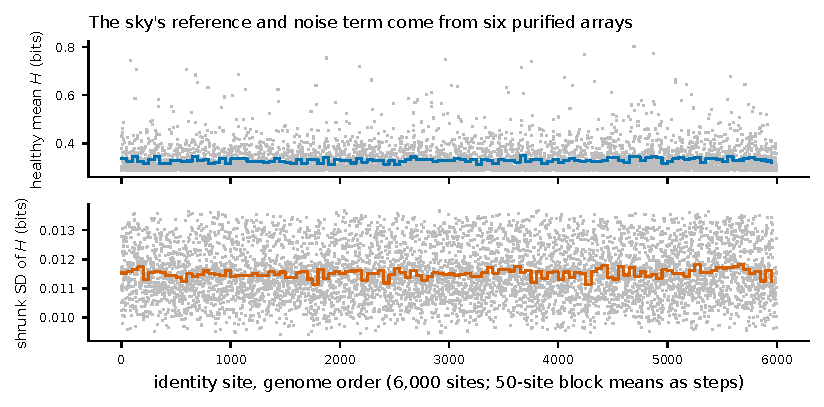
\includegraphics[width=0.95\textwidth]{figures/part6/fig_p4_16_noiseterm.pdf}
\caption{The reference and the noise term of the sky, in genome order over the 6,000 identity sites: healthy mean $H$ (top) and its shrunk SD $s_i$
across the six reference arrays (bottom). Steps: 50-site block means. \calibrated}
\label{fig:p4_noiseterm}
\end{figure}
\begin{table}[htbp]\centering\small
\caption{Inputs of the chain sky (v3 and v4), read from the frozen residual-map reference. \calibrated}\label{tab:p4_skyinputs}
\begin{tabular}{@{}lr@{}}\toprule
quantity & value \\\midrule
identity sites, genome order & 6,000 \\
block size; blocks per map & 10; 600 (50; 120 until 2026-10-09) \\
healthy mean $H$ per site: median (mean) & 0.3133 (0.3303) bits \\
shrunk SD $s_i$: median (range) & 0.0114 (0.0094--0.0137) bits \\
healthy clustering baseline $c_{\rm healthy}$ & 1.0103 (1.1104 at blocks of 50) \\
\bottomrule
\end{tabular}
\end{table}

\section{The whole-array sky}

A sky over every address on the array, not only the identity sites, shows what the cell mix cannot explain anywhere in the genome. The chain now draws it on every report's globe, as a picture from which nothing is scored. The three things it needed are in place: the reference is IAM-Atlas v2.1, with 79 cell types, mixed in the sample's own cell shares as the IAM-Deconvolver reads them; each site's difference is measured in that site's healthy width from the atlas (how much healthy people vary there and how sure the atlas is) and in the sample's own spread, and read in blocks of 10 neighboring sites against a line pure chance crosses less than once in 20 genomes; and the X and Y chromosomes are taken from a frozen list, with every change count also given for them alone, because the atlas's healthy reference pools women and men (Chapter~\ref{ch:skytools}). Scoring a reading from this sky is not commissioned. \openprob

\section{The cell-count floor}

At multipole $\ell$ the CMB offers $2\ell+1$ independent modes, and the fractional uncertainty on the power there can never fall below
$\sqrt{2/(2\ell+1)}$ however good the telescope. A specimen has the same kind of limit. At a site with true methylation $\beta$ in a specimen of $N$
diploid genomes ($2N$ copies of the site), the measured fraction has binomial standard deviation
\begin{equation}
  \sigma_{\mathrm{copies}}=\sqrt{\frac{\beta(1-\beta)}{2N}}
  \label{eq:cellcount}
\end{equation}
for diploid DNA. \derived{} Figure~\ref{fig:cellcount} sets it against array noise. For a whole-blood draw with millions of cells the copy-number floor is
negligible. Plasma cell-free DNA in health carries about $10^3$ genome equivalents per milliliter~\cite{Sender2024}; a genome equivalent is one haploid
genome, one copy of each site, so a draw yields of order $10^3$--$10^4$ copies of a site ($N\approx5\times10^2$--$5\times10^3$). At $10^4$ copies the
floor is $0.0046$ at $\beta=0.7$, below array noise at a single site but not negligible for a cell present at one percent, whose contribution comes
from about a hundred copies. \calc{} The chain does
not yet carry this floor in any interval. \openprob

\begin{figure}[htbp]\centering
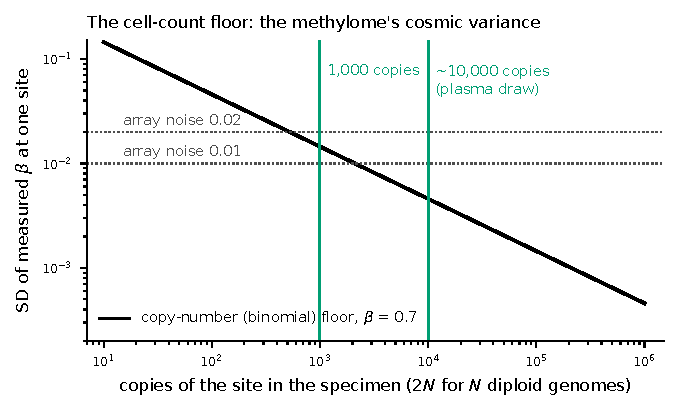
\includegraphics[width=0.8\textwidth]{figures/part6/fig_cell_count_floor.pdf}
\caption{Standard deviation of measured $\beta$ at one site from the finite number of copies of the site (Eq.~\eqref{eq:cellcount} with $2N$ copies, $\beta=0.7$), against
array measurement noise of 0.01 and 0.02. Vertical lines mark $10^3$ and $10^4$ copies (haploid genome equivalents), the range of a plasma draw. \calc}
\label{fig:cellcount}
\end{figure}

\section{A cleaner sky: the out-of-span map}

A residual after composition mixes two things: error in the solved fractions of known cells, and signal from cells the reference does not hold. They can be
separated exactly. Any mixture of the reference's cells, at any fractions, lies in the span of the cells' profiles. Projecting the residual onto that span and
onto its complement,
\begin{equation}
  \mathbf r=\underbrace{P_{\mathrm{span}}\mathbf r}_{\text{composition error}}+\underbrace{(I-P_{\mathrm{span}})\mathbf r}_{\text{what no known mixture can make}},
  \label{eq:outspan}
\end{equation}
leaves an out-of-span map that a composition error cannot move at all. \derived{} It is the direct counterpart of template cleaning on the sky. Its tests are
written before any specimen is projected: a constructed specimen of known cells must read quiet; the map must
stay quiet when the known cells' fractions are thrown off by $\pm50$~\%; cells held out of the reference, spiked in at 1--10~\%, must be detected, in at least 12 of 16 cells at 5~\%; and between two
draws of one person a change of composition must read quiet while a newly added unknown cell appears. \prediction{} The pre-registration is written for the multi-source atlas of
Chapter~\ref{ch:atlas}. The atlas it needs, v2.1, is commissioned, but the map is not built in the chain yet, and the procedure has not run. \openprob
